\documentclass[12pt]{article}
%pdflatex -shell-escape informe.tex 


% --- Paquetes básicos ---
\usepackage[utf8]{inputenc}
\usepackage[T1]{fontenc}
\usepackage[spanish, provide=*]{babel}
\usepackage{geometry}
\usepackage{hyperref}
\geometry{a4paper, margin=2.5cm}
\setlength{\headheight}{14.5pt}
\addtolength{\topmargin}{-2.5pt}

% --- Carátula ---
\title{Python Inicial}
\author{Jose Miguel Paz Portilla\\Pre-Entrega de Proyecto}
\date{\today}

% --- Código Python con minted ---
\usepackage{minted} % Requiere -shell-escape
\usemintedstyle{friendly}

% --- Otros paquetes útiles ---
\usepackage{graphicx}
\usepackage{fancyhdr}
\pagestyle{fancy}
\fancyhead[L]{Python Inicial}
\fancyhead[R]{\thepage}

\begin{document}

% Carátula
\maketitle
\thispagestyle{empty}
\newpage

% Índice
\tableofcontents
\newpage

\section{Introducción}

Con el objetivo de realizar un inventario de productos realizados en python, se realizo una version preliminar con los siguientes requisitos:

\begin{enumerate}
	\item Usar listas para almacenar y gestionar los datos.
	\item Incorporar bucles while y for según corresponda. 
	\item Validar entradas del usuario o usuaria, asegurándote de que no se ingresen datos vacíos o incorrectos.
	\item Utilizar condicionales para gestionar las opciones del menú y las validaciones necesarias.
	\item Presentar un menú que permita elegir entre las funcionalidades disponibles: agregar productos, visualizar productos, buscar productos y eliminar productos.
	\item El programa debe continuar funcionando hasta que se elija una opción para salir.
\end{enumerate}

\section{Implementación}

Utilizo la función main como función principal del programa, el cual muestra un menu con opciones al usuario, y según la opcion elegida realiza alguno de los requisitos solicitados.

Para correr el programa desde una terminal ubicada donde se encuentran los archivos de python y el archivo makefile ingresar \textit{make}, como muesta la \autoref{fig:Correr el programa}

\begin{figure}[H]
	\centering
	\setlength{\fboxrule}{0pt}
	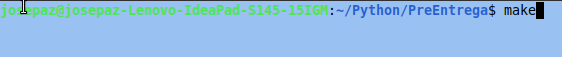
\includegraphics[width=0.66\textwidth]{img7.png}
	\caption{Como correr el programa desde terminal}
	\label{fig:Correr el programa}
\end{figure}  

El programa refresca la terminal y muestra un menu con opciones, se le solicita al usuario que ingrese un número del menu entre las disponibles, como se muestra en la \autoref{fig:menu}.

\begin{figure}[H]
	\centering
	\setlength{\fboxrule}{0pt}
	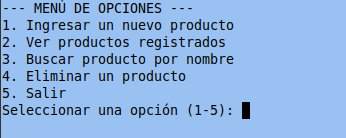
\includegraphics[width=0.4\textwidth]{img1.png}
	\caption{Mostrando el menu}
	\label{fig:menu}
\end{figure} 

Al ingresar la opción $1$, de solicita el nombre, categoria y precio del nuevo producto para almacenarlo en la lista productos, como se muentra en la \autoref{fig:nuevo producto}.

\begin{figure}[H]
	\centering
	\setlength{\fboxrule}{0pt}
	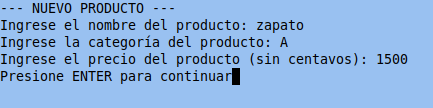
\includegraphics[width=0.5\textwidth]{img2.png}
	\caption{Ingreso nuevo producto}
	\label{fig:nuevo producto}
\end{figure} 

Posteriormente al ingresar la opción $2$, se lista los productos en el inventario, como se muestra en la \autoref{fig:mostrar productos}.

\begin{figure}[H]
	\centering
	\setlength{\fboxrule}{0pt}
	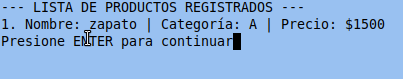
\includegraphics[width=0.5\textwidth]{img3.png}
	\caption{Mostrar productos}
	\label{fig:mostrar productos}
\end{figure} 

Para buscar un producto por su nombre se ingresa la opcion $3$, el programa busca en la lista del inventario y va almacenando en una lista auxiliar todos los productos que coinciden con el nombre del producto, y lo muestra por la terminal, como se muestra en la \autoref{fig:buscar producto}.

\begin{figure}[H]
	\centering
	\setlength{\fboxrule}{0pt}
	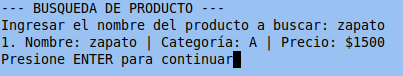
\includegraphics[width=0.5\textwidth]{img4.png}
	\caption{Buscar producto por nombre}
	\label{fig:buscar producto}
\end{figure} 

Con la opción $4$, se puede eliminar un producto con la posición en la lista mostrada por terminal, como se muestra en \autoref{fig:eliminar producto}.

\begin{figure}[H]
	\centering
	\setlength{\fboxrule}{0pt}
	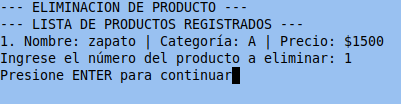
\includegraphics[width=0.5\textwidth]{img5.png}
	\caption{Eliminar producto por indice}
	\label{fig:eliminar producto}
\end{figure} 

Finalmente para finalizar el programa se ingresa la opción $5$, y se muestra por terminal un mensaje de finalización, como en la \autoref{fig:fin programa}.
\begin{figure}[H]
	\centering
	\setlength{\fboxrule}{0pt}
	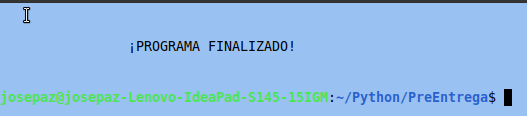
\includegraphics[width=0.66\textwidth]{img6.png}
	\caption{Finalizacion del programa}
	\label{fig:fin programa}
\end{figure} 

\section{makefile}
\inputminted[fontsize=\small]{make}{makefile}

\section{main.py}
\inputminted[fontsize=\small, breaklines=true]{python}{main.py}

\section{menu.py}
\inputminted[fontsize=\small, breaklines=true]{python}{menu.py}

\section{opciones.py}
\inputminted[fontsize=\small, breaklines=true]{python}{opciones.py}

\section{metodos\_productos.py}
\inputminted[fontsize=\small, breaklines=true]{python}{metodos_productos.py}

\section{Conclusión}

En este informe realizado al combinar \LaTeX y Python se presenta una simplificación del programa inventario, donde se pudo aplicar lo aprendido en clases, como listas, condicionales, bucles, ademas se uso modulacion y funciones, además de el uso de la función main y un makefile para ejecutar de un forma más práctica el código.

\end{document}
